\chapter{Relations and Partial Orders}\label{chap:partial_orders}

A relation is a mathematical tool for describing associations between
elements of sets.  Relations are widely used in computer science,
especially in databases and scheduling applications.  A relation can
be defined across many items in many sets, but in this text, we will
focus on \emph{binary} relations, which represent an association
between two items in one or two sets.

\section{Binary Relations}

\subsection{Definitions and Examples}

\begin{definition}\label{def:binary_relation}
Given sets $A$ and~$B$, a \term{binary relation} $R: A \to B$
\emph{from}\footnote{We also say that the relationship is
  \emph{between} $A$ and $B$, or \emph{on}~$A$ if $B = A$.} $A$ to~$B$
is a subset of $A \cross B$.  The sets $A$ and~$B$ are called the
\term{domain} and \term{codomain} of~$R$, respectively.  We commonly
use the notation $aRb$ or $a \sim_R b$ to denote that $(a, b) \in R$.
\end{definition}

A relation is similar to a function.  In fact, every function $f: A
\to B$ is a relation.  In general, the difference between a function
and a relation is that a relation might associate multiple elements
of$B$ with a single element of$A$, whereas a function can only
associate at most one element of~$B$ (namely, $f(a)$) with each
element $a \in A$.

We have already encountered examples of relations in earlier chapters.
For example, in Section~\ref{sexam}, we talked about a relation
between the set of men and the set of women where $mRw$ if man~$m$
likes woman~$w$.  In Section~\ref{sec:coloring}, we talked about a
relation on the set of MIT courses where $c_1 R c_2$ if the exams for
$c_1$ and~$c_2$ cannot be given at the same time.  In
Section~\ref{sec:comm_nets}, we talked about a relation on the set of
switches in a network where $s_1 R s_2$ if $s_1$ and~$s_2$ are
directly connected by a wire.  We did not use the formal definition of
a relation in any of these cases, but they are all examples of
relations.

As another example, we can define an ``in-charge-of'' relation~$T$
from the set of MIT faculty~$F$ to the set of subjects in the 2010 MIT
course catalog.  This relation contains pairs of the form
\[
    (\meta{instructor-name}, \meta{subject-num})
\]
where the faculty member named $\meta{instructor-name}$ is in charge
of the subject with number $\meta{subject-num}$.  So $T$ contains
pairs like those shown in Figure~\ref{fig:7FA}.

\begin{figure}

\begin{tabular}{ll}
(Meyer,    & 6.042),\\
(Meyer,    & 18.062),\\
(Meyer,    & 6.844),\\
(Leighton, & 6.042),\\
(Leighton, & 18.062),\\
(Freeman,  & 6.011),\\
(Freeman,  & 6.881)\\
(Freeman,  & 6.882)\\
(Freeman,  & 6.UAT)\\
(Eng,      & 6.UAT)\\
(Guttag,   & 6.00)
\end{tabular}

\caption{Some items in the ``in-charge-of'' relation~$T$ between
  faculty and subject numbers.}

\label{fig:7FA}

\end{figure}

\dmj{A lot of the MIT-specific stuff should be dropped unless there's
  a clear pedagogic purpose.  For example, do we depend on the fact
  that 6.042 = 18.062?  Do we care that not all MIT faculty are
  mentioned because some are only in charge of Fall courses?  Do we
  care who the Department Education Officer is?}
%
This is a surprisingly complicated relation: Meyer is in charge of
subjects with three numbers.  Leighton is also in charge of subjects
with two of these three numbers---because the same subject,
Mathematics for Computer Science, has two numbers: 6.042 and 18.062,
and Meyer and Leighton are jointly in-charge-of the subject.  Freeman
is in-charge-of even more subjects numbers (around 20), since as
Department Education Officer, he is in charge of whole blocks of
special subject numbers.  Some subjects, like 6.844 and 6.00 have only
one person in-charge.  Some faculty, like Guttag, are in-charge-of
only one subject number, and no one else is jointly in-charge-of his
subject, 6.00.

Some subjects in the codomain, $N$, do not appear in the list ---that
is, they are not an element of any of the pairs in the graph of $T$;
these are the Fall term only subjects.  Similarly, there are faculty
in the domain, $F$, who do not appear in the list because all their
in-charge-of subjects are Fall term only.

\subsection{Representation as a Bipartite Graph}

Every relation $R: A \to B$ can be easily represented as a bipartite
graph $G = (V, E)$ by creating a ``left'' node for each element of~$A$
and a ``right'' node for each element of~$B$.  We then create an edge
between a left node~$u$ and a right node~$v$ whenever $a R b$.
Similarly, every bipartite graph (and every partition of the nodes
into a ``left'' and ``right'' set for which no edge connects a pair of
left or right nodes) determines a relation between the nodes on the
left and the nodes on the right.

For example, we have shown part of the bipartite graph for the
in-charge-of relation from Figure~\ref{fig:7FA} in
Figure~\ref{fig:7FB}.  In this case, there is an edge between
$\meta{instructor-name}$ and $\meta{subject-number}$ if
$\meta{instructor-name}$ is in charge of $\meta{subject-number}$.

\begin{figure}

\gnote{Figure FB, p. 7-7, flt-ch7-jul2.}

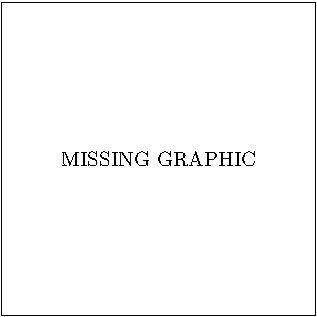
\includegraphics{missing}

\caption{Part of the bipartite graph for the ``in charge of''
  relation~$T$ from Figure~\ref{fig:7FA}.}

\label{fig:7FB}

\end{figure}

\dmj{Do you need to be explicit about assuming $A$ and $B$ are
  finite(?) and that you're imposing an arbitrary order on them?
  Especially since you use a relation on the reals later.}

A relation $R: A \to B$ can also be represented as a matrix $A =
\set{a_{ij}}$ where
\begin{equation*}
    a_{ij} = \begin{cases}
                1 & \text{if the $i$th element of~$A$ is related to
                          the $j$th element of~$B$} \\
                0 & \text{otherwise}
             \end{cases}
\end{equation*}
for $1 \le i \le \card{A}$ and $1 \le j \le \card{B}$.  For example,
the matrix for the relation in Figure~\ref{fig:7FB} (but restricted to
the five faculty and eight subject numbers shown in
Figure~\ref{fig:7FB}, ordering them as they appear top-to-bottom in
Figure~\ref{fig:7FB}) is shown in Figure~\ref{fig:7FC}.

\begin{figure}

\begin{equation*}
\begin{pmatrix}
    1 & 1 & 1 & 0 & 0 & 0 & 0 & 0 \\
    1 & 1 & 0 & 0 & 0 & 0 & 0 & 0 \\
    0 & 0 & 0 & 1 & 1 & 1 & 1 & 0 \\
    0 & 0 & 0 & 0 & 0 & 0 & 1 & 0 \\
    0 & 0 & 0 & 0 & 0 & 0 & 0 & 1
\end{pmatrix}
\end{equation*}

\caption{The matrix for the ``in charge of'' relation~$T$ restricted
  to the five faculty and eight subject numbers shown in
  Figure~\ref{fig:7FB}.  The $(3,4)$ entry of this matrix is~$1$ since
  the third professor (Freeman) is in charge of the fourth subject
  number (6.011).}

\label{fig:7FC}

\end{figure}

\subsection{Relational Images}

The idea of the image of a set under a function extends directly to
relations.

\begin{definition}
The \term{image} of a set~$Y$ under a relation $R: A \to B$, written
$R(Y)$, is the set of elements that are related to some element
in~$Y$, namely,
\begin{equation*}
    R(Y) ::= \set{\, b \in B \mid \text{$y R b$ for some $y \in Y$} \,}.
\end{equation*}
The image of the domain, $R(A)$, is called the \term{range} of~$R$.
\end{definition}

For example, to find the subject numbers that Meyer is in charge of,
we can look for all the pairs of the form
\begin{equation*}
    (\text{Meyer}, \meta{subject-number})
\end{equation*}
in the graph of the teaching relation~$T$, and then just list the
right-hand sides of these pairs.  These right-hand sides are exactly
the image $T(\text{Meyer})$, which happens to be $\set{6.042, 18.062,
  6.844}$.  Similarly, since the domain~$F$ is the set of all
in-charge faculty, $T(F)$, the range of~$T$, is exactly the set of
\emph{all} subjects being taught.

\subsection{Inverse Relations and Images}

\begin{definition}\label{def:inverse}
The \emph{inverse} $\inv{R}$ of a relation $R: A \to B$ is the
relation from~$B$ to~$A$ defined by the rule
\begin{equation*}
    b \inv{R} a \text{ if and only if } a R b.
\end{equation*}
The image of a set under the relation~$\inv{R}$ is called the
\term{inverse image} of the set.  That is, the inverse image of a
set~$X$ under the relation~$R$ is $\inv{R}(X)$.
\end{definition}

Continuing with the in-charge-of example above, we can find the
faculty in charge of 6.UAT by taking the pairs of the form
\begin{equation*}
    (\meta{instructor-name}, \text{6.UAT})
\end{equation*}
for the teaching relation~$T$, and then just listing the left-hand
sides of these pairs; these turn out to be just Eng and Freeman.
These left-hand sides are exactly the inverse image
of~$\set{\text{6.UAT}}$ under~$T$.

Now let $D$ be the set of introductory subjects.  These are the
subjects that have an~0 immediately following the decimal point.  Now
we can likewise find all the instructors who were in-charge-of
introductory subjects by taking all pairs of the form
$(\meta{instructor-name}, \set{1.0\dots, 2.0\dots, 3.0\dots, \dots})$
and list the left-hand sides of these pairs.  These left-hand sides
are exactly the inverse image of~$D$ under~$T$.  From the part of~$T$
show above, we can see that
\begin{equation*}
    \set{ \text{Meyer}, \text{Leighton}, \text{Freeman}, \text{Guttag} }
    \subseteq \inv{T}(D).
\end{equation*}
That is, Meyer, Leighton, Freeman, and Guttag are among the
instructors in charge of introductory subjects.  Finally, the inverse
image under~$T$ of the set~$N$ of all subject numbers is the set of
all instructors who are in charge of a subject.

It gets interesting when we write composite expressions mixing images,
inverse images, and set operations.  For example, $T(\inv{T}(D))$ is
the set of subjects that have an instructor in charge who is also in
charge of an introductory subject.  So $T(\inv{T}(D)) - D$ is the set
of advanced subjects with someone in-charge who is also in-charge-of
an introductory subject.  Similarly, $\inv{T}(D) \intersect
\inv{T}(N - D)$ is the set of faculty in charge of both an
introductory \emph{and} an advanced subject.

\subsection{Surjective and Injective Relations}

There are some properties of relations that will be useful when we
take up the topic of counting in Part~\ref{part:counting} because they
imply certain relations between the \emph{sizes} of domains and
codomains.  In particular, we say that a binary relation $R: A \to B$
is
\begin{itemize}

\item
\term{surjective} if every element of~$B$ is mapped \emph{at least
  once}; more concisely, $R$ is surjective iff $R(A) = B$ (\ie if the
    range of~$R$ is the codomain of~$R$),

\item
\term{total} when every element of~$A$ is assigned to some element
of~$B$; more concisely, $R$ is total iff $A = \inv{R}(B)$,

\item 
\term{injective} if every element of~$B$ is mapped \emph{at most
  once}, and

\item
\term{bijective} if $R$ is total, surjective, injective, and a
function\footnote{These words \emph{surjective}, \emph{injective}, and
  \emph{bijective} are not very memorable.  Some authors use the
  possibly more memorable phrases \term{onto} for surjective,
  \emph{one-to-one} for injective, and \emph{exact correspondence} for
  bijective.}.

\end{itemize}

We can illustrate these properties of a relation $R: A \to B$ in terms
of the corresponding bipartite graph~$G$ for the relation, where nodes
on the left side of~$G$ correspond to elements of~$A$ and nodes on the
right side of~$G$ correspond to elements of~$B$.  For example:
\begin{itemize}

\item
``$R$ is a function'' means that every node on the left is incident to
  \emph{at most} one edge.

\item
``$R$ is total'' means that \emph{every} node on the left is incident
  to \emph{at least} one edge.  So if $R$ is a function, being total
  means that every node on the left is incident to exactly one edge.

\item
``$R$ is surjective'' means that \emph{every} node on the right is
  incident to \emph{at least} one edge.

\item
``$R$ is injective'' means that \emph{every} node on the right is
  incident to \emph{at most} one edge.

\item
``$R$ is bijective'' means that every node on both sides is incident
  to \emph{precisely} one edge (\ie that there is a perfect matching
  between $A$ and~$B$).

\end{itemize}

For example, consider the relations $R_1$ and~$R_2$ shown in
Figure~\ref{fig:7FD}. $R_1$ is a total surjective function (every node
int he left column is incident to exactly one edge, and every node in
the right column is incident to at least one edge), but not injective
(node~3 is incident to 2 edges).  $R_2$ is a total injective function
(every node in the left is incident to exactly one edge, and every
node in the right column is incident to at most one edge), but not
surjective (node~4 is not incident to any edges).

Notice that we need to know what the domain is to determine whether a
relation is total, and we need to know the codomain to determine
whether it's surjective.  For example, the function defined by the
formula~$1/x^2$ is total if its domain is~$\reals^+$ but partial if its
domain is some set of real numbers that includes~0.  It is bijective
if its domain and codomain are both~$\reals^+$, but neither injective
nor surjective it is domain and codomain are both~$\reals$.

\begin{figure}

\gnote{Figure FD, page 7-14, ftl-ch7-jul2.}

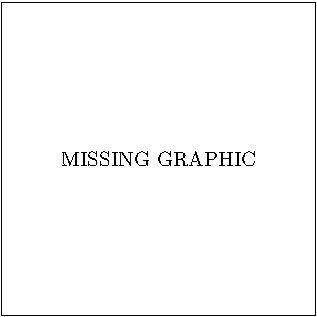
\includegraphics{missing}

\caption{Relation $R_1: A_1 \to B_1$ is shown in~(a) and relation
  $R_2: A_2 \to B_2$ is shown in~(b).}

\label{fig:7FD}

\end{figure}

\subsection{Combining Relations}

There are at least two natural ways to combine relations to form new
relations.  For example, given relations $R : B \to C$ and $S : A \to
B$, the \term{composition} of $R$ with~$S$ is the relation $(R \comp
S) : A \to C$ defined by the rule
\dmj{Should $::=$ be ``iff''}
\begin{equation*}
    a (R \comp S) c ::= \exists b \in B. \; (b R c) \QAND (a S b)
\end{equation*}
where $a \in A$ and $c \in C$.

As a special case, the composition of two functions $f: B \to C$ and
$g: A \to B$ is the function $f \comp g : A \to C$ defined by
\begin{equation*}
    (f \comp g)(a) = f(g(a))
\end{equation*}
for all $a \in A$.  For example, if $A = B = C = \reals$, $g(x) = x +
1$ and $f(x) = x^2$, then
\begin{align*}
    (f \comp g)(x) &= (x + 1)^2 \\
                   &= x^2 + 2x + 1.
\end{align*}

One can also define the \term{product} of two relations $R_1 : A_1 \to
B_1$ and $R_2 : A_2 \to B_2$ to be the relation $S = R_1 \cross R_2$
where
\begin{equation*}
    S : A_1 \cross A_2 \to B_1 \cross B_2
\end{equation*}
and
\begin{equation*}
    (a_1, a_2) S (b_1, b_2) \qiff a_1 R_1 b_1 \text{ and } a_2 R_2 b_2.
\end{equation*}

\section{Relations on One Set}

For the rest of this chapter, we are going to focus on relationships
between elements of a single set; that is, relations from a set $A$ to
a set~$B$ where $A = B$.  Thus, a relation on a set$A$ is a subset $R
\subseteq A \cross A$.  Here are some examples:
\begin{itemize}

\item
Let $A$ be a set of people and the relation$R$ describe who likes
whom: that is, $(x, y) \in R$ if and only if $x$ likes~$y$.

\item
Let $A$ be a set of cities.  Then we can define a relation~$R$ such
that $x R y$ if and only if there is a nonstop flight from city~$x$ to
city~$y$.

\item
Let $A = \integers$ and let $x R y$ hold if and only if $x \equiv y
\pmod{5}$.

\item
Let $A = \naturals$ and let $x R y$ if and only if $x \divides y$.

\item
Let $A = \naturals$ and let $x R y$ if and only if $x \le y$.

\end{itemize}
The last examples clarify the reason for using $x R y$ or $x \sim_R y$
to indicate that the relation~$R$ holds between $x$ and~$y$: many
common relations ($<$, $\le$, $=$, $\divides$, $\equiv$) are expressed
with the relational symbol in the middle.

\subsection{Representation as a Digraph}

Every relation on a single set~$A$ can be modeled as a directed graph
(albeit one that may contain loops).  For example, the graph in
Figure~\ref{fig:7FE} describes the ``likes'' relation for a particular
set of 3 people.

\begin{figure}

\gnote{Figure FE, page 7-19, ftl-ch7-jul2}

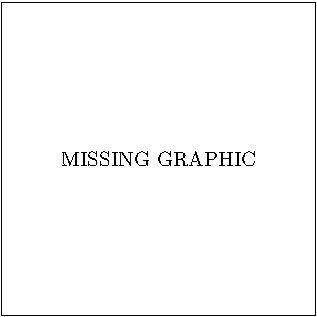
\includegraphics{missing}

\caption{The directed graph for the ``likes'' relation on the set
  $\set{ \text{Bill}, \text{Bob}, \text{Julie} }$.}

\label{fig:7FE}

\end{figure}

In this case, we see that:
\begin{itemize}

\item
Julie likes Bill and Bob, but not herself.

\item
Bill likes only himself.

\item
Bob likes Julie, but not Bill nor himself.

\end{itemize}
Everything about the relationship is conveyed by the directed graph
and nothing more.  This is no coincidence; a set~$A$ together with a
relation~$R$ is precisely the same thing as directed graph $G = (V,
E)$ with vertex set $V = A$ and edge set $E = R$ (where $E$ may have
loops).

As another example, we have illustrated the directed graph for the
divisibility relationship on the set $\set{1, 2, \dots, 12}$ in
Figure~\ref{fig:7FF}.  In this graph, every node has a loop (since
every positive number divides itself) and the composite numbers are
the nodes with indegree more than~1 (not counting the
loop).\dmj{Easier to just say ``greater than~2''?}

\begin{figure}

\gnote{Figure FF, p. 7-21, ftl-ch7-jul2.  Redraw in standard format
  with solid nodes and labels next to the nodes.}

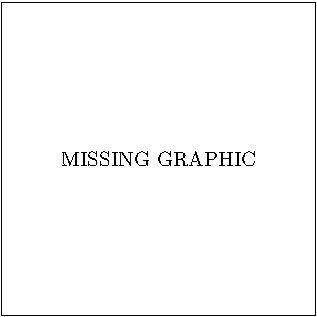
\includegraphics{missing}

\caption{The digraph for divisibility on~$\set{1, 2, \dots, 12}$.}

\label{fig:7FF}

\end{figure}

Relations on a single set can also be represented as a $0, 1$-matrix.
In this case, the matrix is identical to the adjacency matrix for the
corresponding digraph.  For example, the matrix for the relation shown
in Figure~\ref{fig:7FE} is simply
\begin{equation*}
    \begin{pmatrix}
        0 & 1 & 1 \\
        0 & 1 & 0 \\
        1 & 0 & 0
    \end{pmatrix}
\end{equation*}
where $v_1 = \text{Julie}$, $v_2 = \text{Bill}$, and $v_3 =
\text{Bob}$.

\subsection{Symmetry, Transitivity, and Other Special Properties}

Many relations on a single set that arise in practice possess one or
more noteworthy properties.  These properties are summarized in the
box on the following page.  In each case, we provide the formal of the
definition of the property, explain what the property looks like in a
digraph~$G$ for the relation, and give an example of what the property
means for the ``likes'' relation.

\begin{figure}[p]

\textbox{
\textboxtitle{Properties of a Relation $R: A \to A$}

\begin{description}

\item[Reflexivity]

$R$ is \term{reflexive} if $\forall x \in A. \; x R X$.

``Everyone likes themselves.''

Every node in~$G$ has a loop.

\item[Irreflexivity]

$R$ is \term{irreflexive} if $\neg \exists x \in A. \; x R x$.

``No one likes themselves.''

There are no loops in~$G$.

\item[Symmetry]

$R$ is \term{symmetric} if $\forall x, y \in A. \; x R y \QIMP y R x$.

``If $x$ likes~$y$, then $y$ likes~$x$.''

If there is an edge from $x$ to~$y$ in~$G$, then there is an edge from
$y$ to~$x$ in~$G$ as well.

\item[Antisymmetry]

$R$ is \term{antisymmetric} if $\forall x, y \in A\; (x R y \QAND y R
  x) \QIMPLIES x = y$.

``No pair of distinct people like each other.''

There is at most one directed edge between any pair of distinct nodes.

\item[Asymmetry]

$R$ is \emph{asymmetric} if $\neg \exists x, y \in A. \; x R y \QAND
  y R x$.

``No one likes themselves and no pair of people like each other.''

There are no loops and there is at most one directed edge between any
pair of nodes.

\item[Transitivity]

$R$ is \term{transitive} if $\forall x, y, z \in A. \; (x R y \QAND y
  R z) \QIMPLIES x R z$.

``If $x$ likes~$y$ and $y$ likes~$z$, then $x$ likes~$z$ too.''

For any walk $v_0, v_1, \dots, v_k$ in~$G$ where $k \ge 2$,
\ $\diredge{v_0}{v_k}$ is in~$G$ (and, hence, $\diredge{v_i}{v_j}$ is
also in~$G$ for all $i < j$.

\end{description}}

\end{figure}

For example, the congruence relation modulo~5 on~$\integers$ is
reflexive symmetric, and transitive, but not irreflexive,
antisymmetric, or asymmetric.  The same is true for the ``connected''
relation $R: V \to V$ on an undirected graph $G = (V, E)$ where $u R
v$ if $u$ and~$v$ are in the same connected component of graph~$G$.
In fact, relations that have these three properties are so common that
we give them a special name: \term{equivalence relations}.  We will
discuss them in greater detail in just a moment.

As another example, the ``divides'' relation on~$\posints$ is
reflexive, antisymmetric, and transitive, but not irreflexive,
symmetric, or asymmetric.  The same is true for the ``$\le$'' relation
on~$\reals$.  Relations that have these three properties are also very
common and they fall into a special case of relations called a
\term{partial order}.  We will discuss partial orders at length in
Sections \ref{sec:partial_orders}--\ref{sec:dilworth}.

As a final example, consider the ``likes'' relation on the set $\set{
  \text{Julie}, \text{Bill}, \text{Bob} }$ illustrated in
Figure~\ref{fig:7FE}.  This relation has \emph{none} of the six
properties described in the box.

\section{Equivalence Relations}

A relation is an \term{equivalence relation} if it is reflexive,
symmetric, and transitive.  Congruence modulo~$n$ is an excellent
example of an equivalence relation:
\begin{itemize}

\item
It is reflexive because $x \equiv x \pmod{n}$.

\item
It is symmetric because $x \equiv y \pmod{n}$ implies $y \equiv x
\pmod{n}$.

\item
It is transitive because $x \equiv y \pmod{n}$ and $y \equiv z
\pmod{n}$ imply that $x \equiv z \pmod{n}$.

\end{itemize}
There is an even more well-known example of an equivalence relation:
equality itself.  Thus, an equivalence relation is a relation that
shares some key properties with~``$=$''.

\subsection{Partitions}

There is another way to think about equivalence relations, but we'll
need a couple of definitions to understand this alternative
perspective.

\begin{definition}\label{def:equiv_class}

Given an equivalence relation $R : A \to A$, the \term{equivalence
  class} of an element $x \in A$  is the set of all elements of~$A$
related to~$x$ by~$R$.  The equivalence class of~$x$ is
denoted~$[x]$.  Thus, in symbols:
\begin{equation*}
    [x] = \set{\, y \mid x R y \,}.
\end{equation*}
\end{definition}

For example, suppose that $A = \integers$ and $x R y$ means that $x
\equiv y \pmod{5}$.  Then
\begin{equation*}
    [7] = \set{ \dots, -3, 2, 7, 12, 22, \dots }.
\end{equation*}
Notice that 7, 12, 17, etc., all have the same equivalence class; that
is, $[7] = [12] = [17] = \cdots$.

\begin{definition}\label{def:partition}

A \term{partition} of a set~$A$ is a collection of disjoint, nonempty
subsets $A_1$, $A_2$, \dots, $A_n$\dmj{``$A_n$'' implies the partition
  is finite?} whose union is all of~$A$.  The subsets are usually
called the \term{blocks} of the partition.\footnote{We think they
  should be called the \emph{parts} of the partition. Don't you think
  that makes a lot more sense?}  For example, one possible partition
of $A = \set{a, b, c, d, e}$ is
\begin{equation*}
    A_1 = \set{a, c}
    \qquad
    A_2 = \set{b, e}
    \qquad
    A_3 = \set{d}.
\end{equation*}
\end{definition}

Here's the connection between all this stuff: there is an exact
correspondence  between \emph{equivalence relations on~$A$} and
\emph{partitions of~$A$}.  We can state this as a theorem:

\begin{theorem}
The equivalence classes of an equivalence relation on a set~$A$ form a
partition of~$A$.
\end{theorem}

We won't prove this theorem (too dull even for us!), but let's look at
an example.  The congruent-mod-5 relation partitions the integers into
five equivalence classes:
\begin{gather*}
    \set{ \dots, -5, 0, 5, 10, 15, 20, \dots } \\
    \set{ \dots, -4, 1, 6, 11, 16, 21, \dots } \\
    \set{ \dots, -3, 2, 7, 12, 17, 22, \dots } \\
    \set{ \dots, -2, 3, 8, 13, 18, 23, \dots } \\
    \set{ \dots, -1, 4, 9, 14, 19, 24, \dots } \\
\end{gather*}
In these terms, $x \equiv y \pmod{5}$ is equivalent to the assertion
that $x$ and~$y$ are both in the same block of this partition.  For
example, $6 \equiv 16 \pmod{5}$, because they're both in the second
block, but $2 \nequiv 9 \pmod{5}$ because 2~is in the third block
while 9~is in the last block.

In social terms, if ``likes'' were an equivalence relation, then
everyone would be partitioned into cliques of friends who all like
each other and no one else.

\section{Partial Orders}\label{sec:partial_orders}

\subsection{Strong and Weak Partial Orders}

\begin{definition}\label{def:weak_po}

A relation $R$ on a set~$A$ is a \term{weak partial order} if it is
transitive, antisymmetric, and reflexive.  The relation is said to be
a \term{strong partial order} if it is transitive, antisymmetric, and
irreflexive.\footnote{Equivalently, the relation is transitive and
  asymmetric, but stating it this way might have obscured the
  irreflexivity property.}

\end{definition}

Some authors defined partial orders to be what we call weak partial
orders, but we'll use the phrase \emph{partial order} to mean either a
weak or a strong partial order.  The difference between a weak partial
order and a strong one has to do with the reflexivity property: in a
weak partial order, \emph{every} element is related to itself, but in
a strong partial order, \emph{no} element is related to itself.
Otherwise, they are the same in that they are both transitive and
antisymmetric.

Examples of weak partial orders include ``$\le$'' on~$\reals$,
\ ``$\subseteq$'' on the set of subsets of (say)~$\integers$, and the
``divides'' relation on~$\integers$.  Examples of strict partial
orders include~``$<$'' on~$\reals$, and ``$\subset$'' on the set of
subsets of~$\integers$.\footnote{If you are not feeling comfortable
  with all the definitions that we've been throwing at you, it's
  probably a good idea to verify that each of these relations are
  indeed partial orders by checking that they have the transitivity
  and antisymmetry properties.}

We often denote a weak partial order with a symbol such as $\preceq$
or~$\sqsubseteq$ instead of a letter such as~$R$.    This makes sense
from one perspective since the symbols call to mind $\le$
and~$\subseteq$, which define common partial orders.  On the other
hand, a partial order is really a set of related pairs of items, and
so a letter like~$R$ would be more normal.

Likewise, we will often use a symbol like $\prec$ or~$\sqsubset$ to
denote a strong partial order.

\subsection{Total Orders}

A partial order is ``partial'' because there can be two elements with
no relation between them.  For example, in the ``divides'' partial
order on~$\set{1, 2, \dots, 12}$, there is no relation between 3 and~5
(since neither divides the other).

In general, we say that two elements o $a$ and $b$ in a \dmj{You don't
  define ``poset'' until the next section.}poset are
\term{incomparable} if neither $a \preceq b$ nor $b \preceq a$.
Otherwise, if $a \preceq b$ or $b \preceq a$, then we say that $a$
and~$b$ are \term{comparable}.

\begin{definition}\label{def:total_order}
A \term{total order} is a partial order in which every pair of
distinct elements is comparable.
\end{definition}

For example, the ``$\le$'' partial order on~$\reals$ is a total order
because for any pair of real numbers $x$ and~$y$, either $x \le y$ or
$y \le x$.  The ``divides'' partial order on $\set{1, 2, \dots, 12}$
is not a total order because $3 \ndivides 5$ and $5 \ndivides 3$.

\section{Posets and DAGs}

\subsection{Partially Ordered Sets}

\begin{definition}\label{def:poset}
Given a partial order $\preceq$ on a set~$A$, the pair $(A, \preceq)$
is called a \term{partially ordered set} or \term{poset}.
\end{definition}

In terms of graph theory, a poset is simply the directed graph $G =
(A, \preceq)$ with vertex set~$A$ and edge set~$\preceq$.  For example,
Figure~\ref{fig:7FF} shows the graph form of the poset for the
``divides'' relation on~$\set{1, 2, \dots, 12}$.  We have shown the
graph form of the poset for the ``$<$''-relation on $\set{1, 2, 3, 4}$
in Figure~\ref{fig:7FH}.

\begin{figure}

\gnote{Figure FH, p. 7-32, ftl-ch7-jul2.}

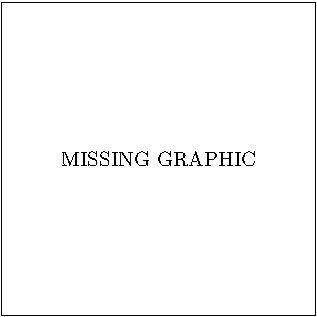
\includegraphics{missing}

\caption{Representing the poset for the ``$<$''-relation on $\set{1,
    2, 3, 4}$ as a digraph.}

\label{fig:7FH}

\end{figure}

\subsection{Posets Are Acyclic}

Did you notice anything that is common to Figures \ref{fig:7FF}
and~\ref{fig:7FH}?  Of course, they both exhibit the transitivity and
antisymmetry properties.  And, except for the loops in
Figure~\ref{fig:7FF}, they both do not contain any cycles.  This is
not a coincidence.  In fact, the combination of the transitivity and
asymmetry properties imply that the digraph for any poset is an
acyclic graph (\ie a DAG), at least if you don't count loops as
cycles.  We prove this fact in the following theorem.

\begin{theorem}\label{thm:poset=acyclic}
A poset has no directed cycles other than self-loops.
\end{theorem}

\begin{proof}

We use proof by contradiction.  Let $(A, \preceq)$ be a poset.
Suppose that there exist $n \ge 2$ distinct elements $a_1$, $a_2$,
\dots, $a_n$ such that
\begin{equation*}
    a_1 \preceq a_2 \preceq a_3 \preceq \dots \preceq a_{n - 1}
    \preceq a_n \preceq a_1.
\end{equation*}
Since $a_1 \preceq a_2$ and $a_2 \preceq a_3$, transitivity implies
$a_1 \preceq a_3$.  Another application of transitivity shows that
$a_1 \preceq a_4$ and a routine induction argument establishes that
$a_1 \preceq a_n$.  Since we know that $a_n \preceq a_1$, antisymmetry
implies $a_1 = a_n$, contradicting the supposition that $a_1$, \dots,
$a_n$ are distinct and $n \ge 2$.  Thus, there is no such directed
cycle.
\end{proof}

Thus, deleting the self-loops from a poset leaves a directed graph
without cycles, which makes it a \term{directed acyclic graph} or
\term{DAG}.

\subsection{Transitive Closure}

Theorem~\ref{thm:poset=acyclic} tells us that every poset corresponds
to a~DAG\@.  Is the reverse true?  That is, does every DAG correspond
to a poset?  The answer is ``Yes,'' but we need to modify the DAG to
make sure that it satisfies the transitivity property.  For example,
consider the DAG shown in Figure~\ref{fig:7FJ}.  As any DAG must, this
graph satisfies the antisymmetry property\footnote{If
  $\diredge{u}{v}$ and $\diredge{v}{u}$ are in a digraph~$G$, then $G$
would have a cycle of length~2 and it could not be a DAG.} but it does
not satisfy the transitivity property because $\diredge{v_1}{v_2}$ and
$\diredge{v_2}{v_3}$ are in the graph but $\diredge{v_1}{v_3}$ is not
in the graph.

\begin{figure}

\gnote{Figure FJ, p. 7-34, ftl-ch7-jul7.}

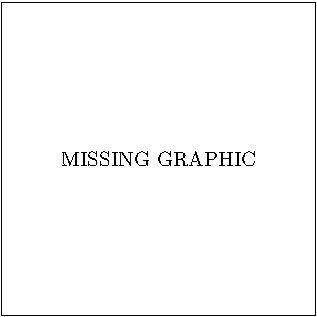
\includegraphics{missing}

\caption{A 6-node digraph that does not satisfy the transitivity
  property.}

\label{fig:7FJ}

\end{figure}

\begin{definition}\label{def:transitive_closure}
Given a digraph $G = (V, E)$, the \term{transitive closure} of~$G$ is
the digraph $G^+ = (V, E^+)$ where
\begin{equation*}
    E^+ = \set{\, \diredge{u}{v} | \text{there is a directed path of
        positive length from $u$ to $v$ in $G$} \,}.
\end{equation*}
Similarly, if $R$ is the relation corresponding to~$G$, the
\term{transitive closure} of~$R$ (denoted~$R^+$ is the relation
corresponding to~$G^+$.
\end{definition}

For example, the transitive closure for the graph in
Figure~\ref{fig:7FJ} is shown in Figure~\ref{fig:7FK}.

\begin{figure}

\gnote{Figure FK, p. 7-36, ftl-ch7-jul2.  Doubled lines should be
  rendered as heavy lines.}

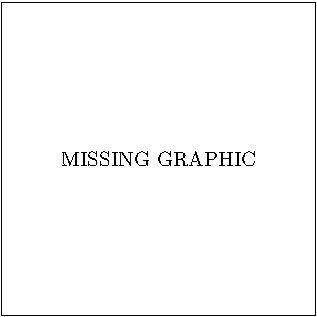
\includegraphics{missing}

\caption{The transitivity closure for the digraph in
  Figure~\ref{fig:7FJ}.  The edges that were added to form the
  transitive closure are shown in bold.}

\label{fig:7FK}

\end{figure}

If $G$ is a DAG, then the transitive closure of~$G$ is a strong
partial order.  The proof of this fact is left as an exercise in the
problem section.

\subsection{The Hasse Diagram}

On problem with viewing a poset as a digraph is that there tend to be
lots of edges due to the transitivity property.  Fortunately, we do
not necessarily have to draw all the edges if we know that the digraph
corresponds to a poset.  For example, we could choose not to draw any
edge which would be implied by the transitivity property, knowing that
it is really there by implication.  In general, a \term{Hasse diagram}
for a poset~$(A, \preceq)$ is a digraph with vertex set~$A$ and edge
set~$\preceq$ minus all self-loops and edges implied by transitivity.
For example, the Hasse diagrams of the posets shown in Figures
\ref{fig:7FF} and~\ref{fig:7FH} are shown in Figure~\ref{fig:7FM}.

\begin{figure}

\gnote{Figure FM, p 7-38, ftl-chap7-jul2.  Render as two figures.}

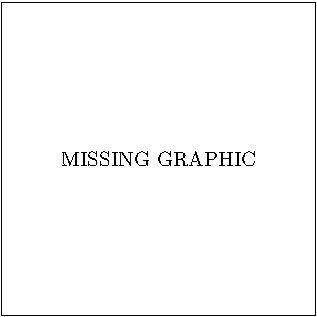
\includegraphics{missing}

\caption{The Hasse diagrams for the posets in Figure \ref{fig:7FF}
  and~\ref{fig:7FH}.}

\label{fig:7FM}

\end{figure}

\section{Topological Sort}

A total order that is consistent with a partial order is called a
topological sort  More precisely, a \term{topological sort} of a
poset~$(A, \preceq)$ is a total order~$(A, \preceq_T)$ such that
\begin{equation*}
    x \preceq y \QIMPLIES x \preceq_T y.
\end{equation*}

For example, consider the poset that describes how a guy might get
dressed for a formal occasion.  The Hasse diagram for such a poset is
shown in Figure~\ref{fig:7FP}.  In this poset, the \emph{set} is all
the garments and the \emph{partial order} specifies which items much
precede others when getting dressed.

\begin{figure}

\gnote{Figure FP, p. 7-40, ftl-ch7-jul2.}

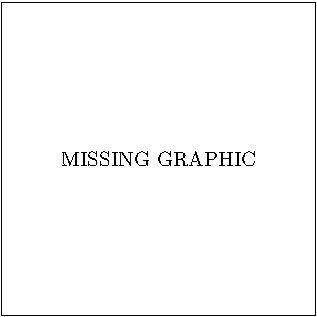
\includegraphics{missing}

\caption{The Hasse diagram for a poset that describes which items much
  precede others when getting dressed.}

\label{fig:7FP}

\end{figure}

There are several total orders that are consistent with the partial
order shown in Figure~\ref{fig:7FP}.  We have shown to of them in list
form in Figure~\ref{fig:7FQ}.  Each such list is a topological sort
for the partial order in Figure~\ref{fig:7FP}.  In what follows, we
will prove that every \emph{finite} poset has a topological sort.  You
can think of this as a mathematical proof that you \emph{can} get
dressed in the morning (and then show up for math lecture).

\begin{figure}

\begin{tabular}{c@{\hspace{4em}}c}
underwear       & left sock \\
pants           & shirt \\
belt            & tie \\
shirt           & underwear \\
tie             & right sock \\
jacket          & pants \\
left sock       & right shoe \\
right sock      & belt \\
left shoe       & jacket \\
right shoe      & left shoe \\[\medskipamount]
(a)             & (b)
\end{tabular}

\caption{Two possible topological sorts of the poset shown in
  Figure~\ref{fig:7FP}.  In each case, the elements are listed so that
  $x \preceq y$ iff $x$ is above~$y$ in the list.}

\label{fig:7FQ}

\end{figure}

\begin{theorem}\label{thm:topological_sort}
Every finite poset has a topological sort.
\end{theorem}

We'll prove the theorem constructively.  The basic idea is to pull the
``smallest'' element~$a$ out of the poset, find a topological sort of
the remainder recursively, and then add~$a$ back into the topological
sort as an element smaller than all the others.

The first hurdle is that ``smallest'' is not such a simple concept in
a set that is only partially ordered.  In a poset~$(A, \preceq)$, an
element $x \in A$ is \term{minimal} if there is no other element $y
\in A$ such that $y \preceq x$.  For example, there are \emph{four}
minimal elements in the getting-dressed poset: left sock, right sock,
underwear, and shirt.  (It may seem odd that the minimal elements are
at the top of the Hasse diagram rather than the bottom.  Some people
adopt the opposite convention.  If you're not sure whether minimal
elements are on the top or bottom in a particular context, ask.)
Similarly, an element $x \in A$ is \term{maximal} if there is no other
element $y \in A$ such that $x \preceq y$.

Proving that every poset \emph{has} a minimal element is extremely
difficult, because this is actually false.  For example, the
poset~$(\integers, \le)$ has no minimal element.  However, there is at
least one minimal element in every \emph{finite} poset.

\begin{lemma}\label{lem:min_element}
Every finite poset has a minimal element.
\end{lemma}

\begin{proof}
Let $(A, \preceq)$ be an arbitrary poset.  Let $a_1$, $a_2$, \dots,
$a_n$ be a maximum-length sequence of distinct elements in~$A$ such
that
\begin{equation*}
    a_1 \preceq a_2 \preceq \dots \preceq a_n.
\end{equation*}
The existence of such a maximum-length sequence follows from the Well
Ordering Principle and the fact that $A$ is finite.  Now $a_0 \preceq
a_1$ cannot hold for any element $a_0 \in A$ not in the chain, since
the chain already has maximum length.  And $a_i \preceq a_1$ cannot
hold for any $i \ge 2$, since that would imply a cycle
\begin{equation*}
    a_i \preceq a_1 \preceq a_2 \preceq \dots \preceq a_i
\end{equation*}
and no cycles exist in a poset by Theorem~\ref{thm:poset=acyclic}.
Therefore $a_1$ is a minimal element.
\end{proof}

Now we're ready to prove Theorem~\ref{thm:topological_sort}, which
says that every finite poset has a topological sort.  The proof is
rather intricate; understanding the argument requires a clear grasp of
all the mathematical machinery related to posets and relations!

\begin{proof}[Proof of Theorem~\ref{thm:topological_sort}]
We use induction.  Let $P(n)$ be the proposition that every
$n$-element poset has a topological sort.

\inductioncase{Base case}: Every 1-element poset is already a total
order and thus is its own topological sort.  So $P(1)$ is true.

\inductioncase{Inductive step}: Now we assume $P(n)$ in order to prove
$P(n + 1)$ where $n \ge 1$.  Let $(A, \preceq)$ be an $(n +
1)$-element poset.  By Lemma~\ref{lem:min_element}, there exists a
minimal element in~$a \in A$.  Remove $a$ and all pairs in~$\preceq$
involving~$a$ to obtain an $n$-element poset~$(A', \preceq')$.  This
has a topological sort~$(A', \preceq'_T)$ by the assumption~$P(n)$.
Now we construct a total order~$(A, \preceq_T)$ by adding $a$ back as
an element smaller than all the others.  Formally, let
\begin{equation*}
    \preceq_T = \preceq'_T \union \set{\, (a, z) \mid z \in A \,}.
\end{equation*}
All that remains is to check that this total order is consistent with
the original partial order~$(A, \preceq)$; that is, we must show that
\begin{equation*}
    x \preceq y \QIMPLIES x \preceq_T y.
\end{equation*}
We assume that the left side is true and show that the right side
follows.  There are two cases.
\begin{description}

\item[Case 1]

If $x = a$, then $a \preceq_T y$ holds, because $a \preceq_T z$ for
all $z \in A$.

\item[Case 2]

if $x \ne a$, then $y$ can not equal $a$ either, since $a$ is a
minimal element in the partial order~$\preceq$.  Thus, both $x$
and~$y$ are in~$A'$ and so $x \preceq' y$.  This means $x \preceq'_T
y$, since $\preceq'_T$ is a topological sort of the partial
order~$\preceq'$.  And this implies $x \preceq_T y$ since $\preceq_T$
contains~$\preceq'_T$.
\end{description}

Thus, $(A, \preceq_T)$ is a topological sort of~$(A, \preceq)$.  This
shows that $P(n)$ implies $P(n + 1)$ for all $n \ge 1$.  Therefore
$P(n)$ is true for all $n \ge 1$ by the principle of induction, which
proves the theorem.
\end{proof}

\section{Parallel Task Scheduling}\label{sec:parallel_task}

When items of a poset are tasks that need to be done and the partial
order is a precedence constraint, topological sorting provides us with
a way to execute the tasks sequentially without violating the
precedence constraints.

But what if we have the ability to execute more than one task at the
same time?  For example, suppose that the tasks are programs, the
partial order indicates data dependence, and we have a parallel
machine with lots of processors instead of a sequential machine with
only one processor.  How should we schedule the tasks so as to
minimize the total time used?

For simplicity, assume all tasks take 1 unit of time and we have an
unlimited number of identical processors.  For example, in the clothes
example in Figure~\ref{fig:7FP}, how long would it take to handle all
the garments?

In the first unit of time, we should do all minimal items, so we would
put on our left sock, our right sock, our underwear, and our shirt.
In the second unit of time, we should put on our pants and our tie.
Note that we cannot put on our left or right shoe yet, since we have
not yet put on our pants.  In the third unit of time, we should put on
our left shoe, our right shoe, and our belt.  Finally, in the last
unit of time, we can put on our jacket.  This schedule is illustrated
in Figure~\ref{fig:7FS}.

\begin{figure}

\gnote{Figure FS, p. 7-44, ftl-ch7-jul2.}

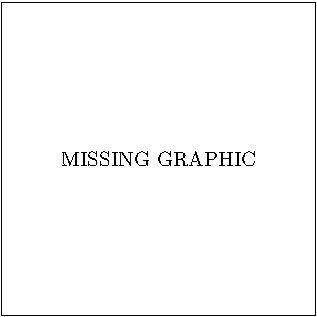
\includegraphics{missing}

\caption{A parallel schedule for the tasks-in-getting-dressed poset in
Figure~\ref{fig:7FP}.  The tasks in~$A_i$ can be performed in step~$i$
for $1 \le i \le 4$.  A chain of length~4 (the critical path in this
example) is shown with bold edges.}

\label{fig:7FS}

\end{figure}

The total time to do these tasks is 4~units.  We cannot do better than
4~units of time because there is a sequence of 4~tasks, each needing
to be done before the next, of length~4.  Here, for example, we must
put on our shirt before our pants, our pants before our  belt, and our
belt before our jacket.  Such a sequence of items is known as a
\term{chain}

\begin{definition}\label{def:chain}
A \term{chain} is a sequence $a_1 \preceq a_2 \preceq \dots \preceq
a_t$, where $a_i \ne a_j$ for all $i \ne j$, such that each item is
comparable to the next in the chain, and it is smaller with respect
to~$\preceq$.  The \term{length} of the chain is~$t$, the number of
elements in the chain.
\end{definition}

Thus, the time it takes to schedule tasks, even with an unlimited
number of processors, is at least the length of the longest chain.
Indeed, if we used less time, then two items from the chain would have
to be done at the same time, which contradicts the precedence
constraints.  For this reason, \dmj{\emph{a} longest chain?}the
longest chain is also known as a \term{critical path}.  For example,
Figure~\ref{fig:7FS} shows the critical path for the getting-dressed
poset.

In this example, we were in fact able to schedule all the tasks in $t$
steps, where $t$ is the length of the longest chain.  The really nice
thing about posets is that this is always possible!  In other words,
for any poset, there is a legal parallel schedule that runs in $t$
steps, where $t$ is the length of the longest chain.

There are lots of ways to prove this fact.  Our proof will also give
us the corresponding schedule in $t$~time steps, and allow us to
obtain some nice corollaries.

\begin{theorem}\label{thm:poset-partition}
Given any finite poset $(A, \preceq)$ for which the longest chain has
length~$t$, it is possible to partition~$A$ into $t$ subsets $A_1$,
$A_2$, \dots, $A_t$ such that for all $i \in \set{1, 2, \dots, t}$ and
for all $a \in A_i$, we have that all $b \preceq a$ appear in the set
$A_1 \union \dots \union A_{i - 1}$.
\end{theorem}

Before proving this theorem, first note that for each~$i$, all items
in~$A_i$ can be scheduled in time step~$i$.  This is because all
preceding tasks are scheduled in preceding time steps, and thus are
already completed.  So the theorem implies that

\begin{corollary}
The total amount of parallel time needed to complete the tasks is the
same as the length of the longest chain.
\end{corollary}

\begin{proof}[Proof of Theorem~\ref{thm:poset-partition}]
For all $a \in A_i$, put $a in A_i$, where $i$~is the length of the
longest chain ending at~$a$.  For example, the $A_i$ for the
getting-dressed poset are shown in Figure~\ref{fig:7FS}.  In what
follows, we show that for all~$i$, for all $a \in A_i$ and for all $b
\preceq a$ with $b \ne a$, we have $b \in A_1 \union A_2 \union \dots
\union A_{i - 1}$.

We prove this by contradiction.  Assume there is some $i$, \ $a \in
A_i$, and $b \preceq a$ with $b \ne a$ and $b \notin A_1 \union A_2
\union \dots \union A_{i - 1}$.  By the way we defined $A_i$, this
implies there is a chain of length at least~$i$ ending at~$b$.  Since
$b \preceq a$ and $b \ne a$, we can extend this chain to a chain of
length at least $i + 1$, ending at~$a$.  But then $a$ could not be
in~$A_i$.  This is a contradiction.
\end{proof}

If we have an unlimited number of processors, then the time to
complete all tasks is equal to the length of the longest chain of
dependent tasks.  The case where there are only a limited number of
processors is covered in the Problems section.


\section{Dilworth's Lemma}\label{sec:dilworth}

\begin{definition}\label{def:antichain}
An \term{antichain} in a partial order is a set of elements such that
any two elements in the set are incomparable.
\end{definition}

For example, each $A_i$ in the proof of
Theorem~\ref{thm:poset-partition} and in Figure~\ref{fig:7FS} is an
antichain since they have no dependencies between them (which is why
they could be executed at the same time).

Our conclusions about scheduling also tell us something about
antichains.

\begin{corollary}\label{cor:antichains}
If the largest chain in a partial order on a set~$A$ is of size~$t$,
then $A$ can be partitioned into $t$~antichains.
\end{corollary}

\begin{proof}
Le the antichains be the sets $A_1$, $A_2$, \dots, $A_t$.
\end{proof}

Corollary~\ref{cor:antichains} implies a famous result\footnote{Lemma
  ~\ref{lem:dilworth} also follows from a more general result known as
  Dilworth's Theorem that we will not discuss.} about partially
ordered sets:

\begin{lemma}\label{lem:dilworth}
For all $t > 0$, every partially ordered set with $n$ elements must
have either a chain of size greater than~$t$ or an antichain of size
at least~$n/t$.
\end{lemma}

\begin{proof}
By contradiction.  Assume that the longest chain has length at
most~$t$ and the longest antichain has size less than~$n/t$.  Suppose
that the largest chain is of size~${}\le t$.  Then
Corollary~\ref{cor:antichains}, the $n$ elements can be partitioned
into at most $t$ antichains.  Hence, there are fewer than $t \cdot n/t
= n$ elements in the poset, which is a contradiction.  Hence there
must be a chain longer than~$t$ or an antichain with at least
$n/t$~elements.
\end{proof}

\begin{corollary}\label{cor:dilworth:sqrtN}
Every partially ordered set with $n$ elements has a chain of size
greater than~$\sqrt{n}$ or an antichain of size at least~$\sqrt{n}$.
\end{corollary}

\begin{proof}
Set $t = \sqrt{n}$ in Lemma~\ref{lem:dilworth}.
\end{proof}

As an application, consider a permutation of the numbers from 1 to~$n$
arranged as a sequence from left to right on a line.
Corollary~\ref{cor:dilworth:sqrtN} can be used to show that there must
be a $\sqrt{n}$-length subsequence of these numbers that is completely
increasing or completely decreasing as you move from left to right.
For example, the sequence
\begin{equation*}
    7, 8, 9, 4, 5, 6, 1, 2, 3
\end{equation*}
has an increasing subsequence of length~3 (for example, 7, 8, 9) and a
decreasing subsequence of length~3 (for example, 9, 6, 3).  The proof
of this result is left as an exercise that will test your ability to
find the right partial order on the numbers in the sequence.

\section{Problems}

\endinput
